\documentclass[a4paper]{scrartcl}
\usepackage[cm]{fullpage}
\usepackage{amsmath, amssymb}
\usepackage{siunitx}
\usepackage{arydshln}

\usepackage{tikz, pgfplots}
\tikzstyle{every node} = [align = center]
\pgfplotsset{
    compat = 1.9,
    graph/.style = {
        axis lines = middle,
        grid = both,
        minor tick num = 3,
        every major grid/.style = {orange, opacity=0.5},
        legend pos = outer north east
    },
    graph-scatter/.style = {
        only marks,
        error bars/.cd,
        x dir = both, y dir = both,
        x explicit, y explicit
    }
}

\begin{document}

\title{PHYS1241: Interference in Thin Films and Ray Optics}
\author{ \\ \\ }
\date{2015-09-17}
\maketitle

\section{Abstract}
Thin film interference is exploited to allow measuring lenses with very large radius of curvatures and transparent planes at very small angles of inclination, with the examples provided found to have a radius of curvature of \SI{596 \pm 92}{\metre} and an angle of inclination of \SI{12.1 \pm 0.2}{\arcsecond}, respectively.

Snell's law was also tested to be correct, producing the refractive index of the material measured to be \SI{1.47 \pm 0.03}{} as a side effect.

\section{Introduction}
Thin film interference is important in several areas, one of which is the measuring of lenses with very large radius of curvatures and small angles of inclination in transparent materials. The first two parts of this experiment is to perform these measurements on two example situations.

Snell's law is important to understanding how light behaves at a boundary condition, and is used to measure the refractive index of materials. The third part of this experiment serves to test Snell's law and verify that it is correct.

\section{Materials and Methods}
Please refer to pages 103 to 105 inclusive in the PHYS1241 laboratory manual for the base materials and methods used. The wavelength of light used for parts 1 and 2 was \(\lambda = \SI{596.3}{\nano\metre}\).

\subsection{Part 1: Newton's Rings}
Using the formulae \(2 t = n \lambda\) and \(2 t R = r^2\) derived in the laboratory manual on pages 99 and 101, respectively, solving for the radius of curvature \(R\) gives \(R = \frac{r^2}{n \lambda}\). Performing a linear regression on data points of \(r^2\) against \(n\) and then dividing the gradient by \(\lambda\) will yield the radius of curvature.

\subsection{Part 2: Air Wedge}
Using the \(t = d \theta\) derived on page 102, solving for \(\theta\) gives \(\theta = \frac{n \lambda}{2 d}\). Since this expression is linear in \(n\) and \(d \theta\), one can take any arbitrary \(\Delta n\) and the corresponding \(\Delta d\) to solve for \(\theta\) through \(\theta = \frac{\lambda \Delta n}{2 \Delta d}\), so knowing what \(n\) is is unnecessary.

\subsection{Part 3: Ray Optics}
Snell's law can be tested for by shining the beam of light at the centre of the lens at various angles, and observing the angle it leaves the lens. This tests the air-to-lens boundary since the light leaves the lens perpendicular to the curved side, so the light is only bent at the air-to-lens boundary. Taking the angle of incidence \(\theta_1\) and refraction \(\theta_2\) pairs, an estimated refractive index for the lens can be calculated using Snell's law. If Snell's law were to hold, this refractive index will stay the same regardless of the angle of incidence, which can be checked by seeing if \(\frac{\sin\theta_2}{\sin\theta_1}\) forms a line.

Additionally, the critical angle for the lens-to-air boundary can be found by shining the light perpendicular to the curved side. This angle can then be compared with the refractive index obtained above using Snell's law to further test it.

\section{Results}
\subsection{Part 1: Newton's Rings}
\begin{table}
    \centering
    \begin{tabular}{c | c | c | c | c}
        \(n\) & Diameter (\si{\milli\metre}) & Inner/Outer diameter (\si{\milli\metre}) & Uncertainty in diameter (\si{\milli\metre}) & Radius (\(r\)) (\si{\milli\metre}) \\
        \hline
        1 & 38.9 & 33.2/44.5 & 5.7 & \SI{19.5 \pm 2.8}{} \\
        2 & 53.6 & 48.5/58.4 & 5.0 & \SI{26.8 \pm 2.5}{} \\
        3 & 64.8 & 60.0/69.7 & 4.9 & \SI{32.4 \pm 2.4}{} \\
        4 & 74.6 & 69.7/79.3 & 4.8 & \SI{37.3 \pm 2.4}{} \\
        5 & 83.1 & 78.3/87.8 & 4.8 & \SI{41.6 \pm 2.4}{} \\
        \hline
    \end{tabular}
    \caption{Part 1 measurements of the dark fringes}
    \label{tab:part1_data}
\end{table}

\begin{figure}
    \centering
    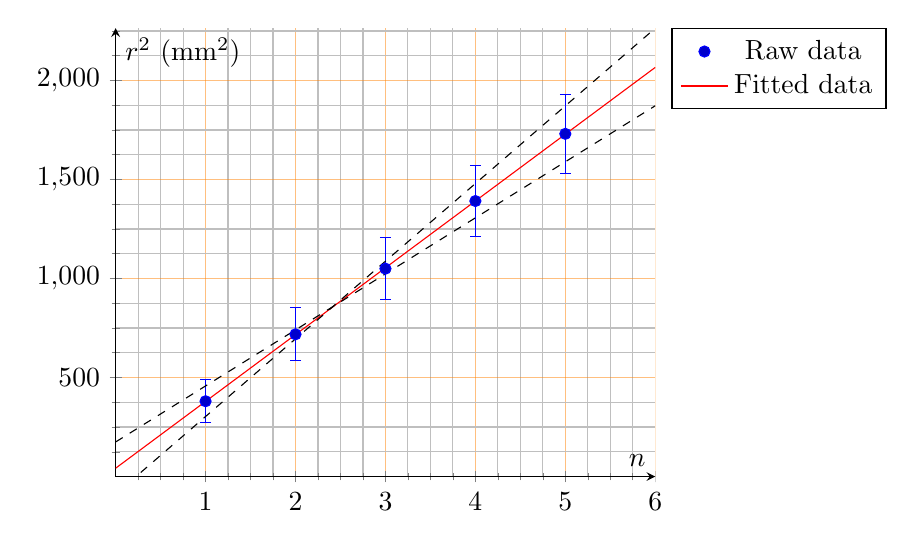
\begin{tikzpicture}
        \begin{axis}[
            graph,
            xlabel = \(n\),
            ylabel = \(r^2\) (\si{\milli\metre\squared}),
            xmin = 0,
            ymin = 0
        ]
            \addplot +[graph-scatter] table [
                y error = yerror
            ] {
                x   y       yerror
                1   380.25  109.2
                2   718.24  134
                3   1049.8  155.52
                4   1391.3  179.04
                5   1730.6  199.68
            };
            \addlegendentry{Raw data}
            
            \addplot +[no marks, domain = 0:6] {41.91 + 337.376 * x};
            \addlegendentry{Fitted data}
            
            \addplot [no marks, dashed, domain = 0:6] {-89.157 + 392.190 * x};
            \addplot [no marks, dashed, domain = 0:6] {174.482 + 282.985 * x};
        \end{axis}
    \end{tikzpicture}
    \caption{Part 1 raw and fitted data}
    \label{fig:part1_graph}
\end{figure}

From the results shown in Table \ref{tab:part1_data}, taking the linear regression (Figure \ref{fig:part1_graph}) gives a gradient of \(\frac{r^2}{n} = \SI{337 \pm 55}{\milli\metre\squared}\). Solving for the radius of curvature then gives \(R = \SI{596 \pm 92}{\metre}\).

\subsection{Part 2: Air Wedge}
\begin{table}
    \centering
    \begin{tabular}{c | c}
        Distance between 10 fringes (\si{\milli\metre}) & Distance between fringes (\si{\milli\metre}) \\
        \hline
        49.9 & 4.99 \\
        50.1 & 5.01 \\
        51.1 & 5.11 \\
        51.6 & 5.16 \\
        51.9 & 5.19 \\
        \hdashline
        \SI{50.9 \pm 1.0}{} & \SI{5.09 \pm 0.10}{} \\
        \hline
    \end{tabular}
    \caption{Part 2 measurements of the dark fringes}
    \label{tab:part2_data}
\end{table}

Using the results shown in Table \ref{tab:part2_data}, we obtain \(\Delta n = 10\) and \(\Delta d = \SI{50.9 \pm 1.0}{\milli\metre}\). Plugging these values directly into \(\theta = \frac{\lambda \Delta n}{2 \Delta d}\) gives \(\theta = \SI{5.86 \pm 0.12e-5}{\radian} = \SI{12.1 \pm 0.2}{\arcsecond}\).

\subsection{Part 3: Ray Optics}
\begin{table}
    \centering
    \begin{tabular}{c | c}
        Incidence (\(\theta_1\)) & Refraction (\(\theta_2\)) \\
        \hline
        \SI{0.0 \pm 0.1}{\degree} & \SI{0.0 \pm 0.1}{\degree} \\
        \SI{20.0 \pm 0.1}{\degree} & \SI{14 \pm 1}{\degree} \\
        \SI{30.0 \pm 0.1}{\degree} & \SI{20 \pm 1}{\degree} \\
        \SI{40.0 \pm 0.1}{\degree} & \SI{28 \pm 1}{\degree} \\
        \SI{50.0 \pm 0.1}{\degree} & \SI{31 \pm 1}{\degree} \\
        \SI{60.0 \pm 0.1}{\degree} & \SI{36 \pm 1}{\degree} \\
        \SI{70.0 \pm 0.1}{\degree} & \SI{39 \pm 1}{\degree} \\
        \SI{80.0 \pm 0.1}{\degree} & \SI{42 \pm 1}{\degree} \\
        \hline
    \end{tabular}
    \caption{Air to Lens refraction data}
    \label{tab:part3_data}
\end{table}

\begin{figure}
    \centering
    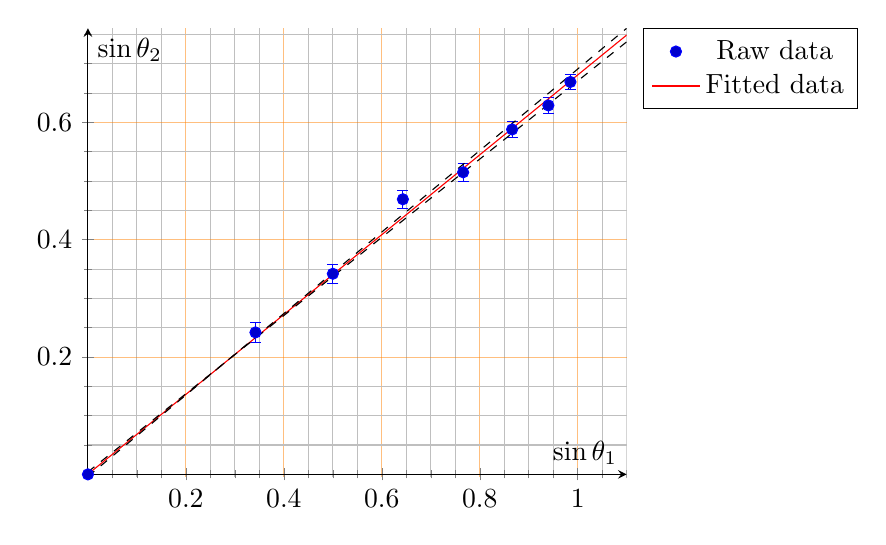
\begin{tikzpicture}
        \begin{axis}[
            graph,
            xlabel = \(\sin\theta_1\),
            ylabel = \(\sin\theta_2\)
        ]
            \addplot +[graph-scatter] table [
                x error = xerror,
                y error = yerror
            ] {
                x       y       xerror  yerror
                0       0       0.00175 0.00175
                0.342   0.242   0.00164 0.0169
                0.5     0.342   0.00151 0.0164
                0.643   0.469   0.00134 0.0154
                0.766   0.515   0.00112 0.015
                0.866   0.588   0.00087 0.0141
                0.94    0.629   0.0006  0.0136
                0.985   0.669   0.0003  0.013
            };
            \addlegendentry{Raw data}
            
            \addplot +[no marks, domain = 0:1.1] {0.000258664 + 0.680714 * x};
            \addlegendentry{Fitted data}
            
            \addplot [no marks, dashed, domain = 0:1.1] {-0.00368148 + 0.694809 * x};
            \addplot [no marks, dashed, domain = 0:1.1] {0.00419881 + 0.666619 * x};
        \end{axis}
    \end{tikzpicture}
    \caption{Part 3 raw and fitted data}
    \label{fig:part3_graph}
\end{figure}

\begin{figure}
    \centering
    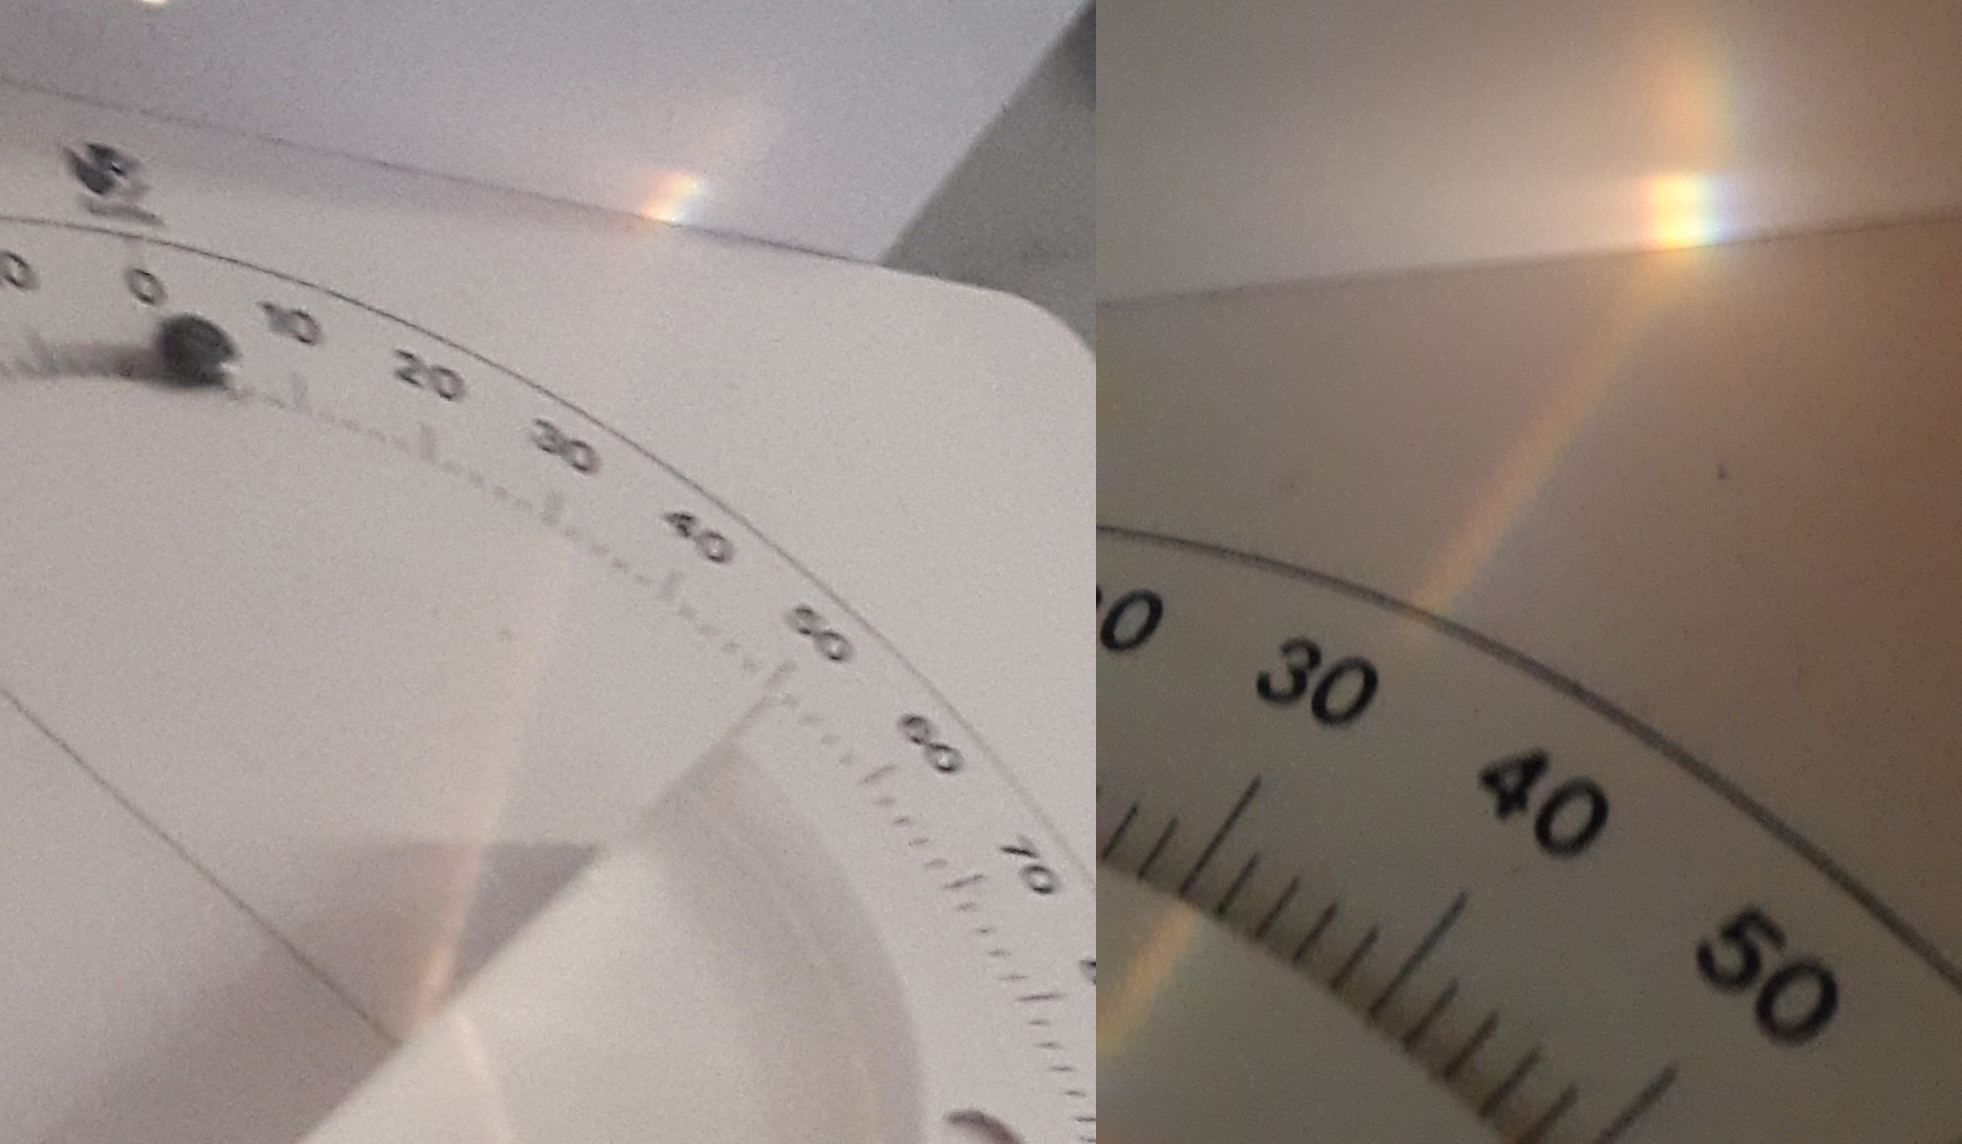
\includegraphics[width = 15cm]{part3.png}
    \caption{Dispersion of light through the lens}
    \label{fig:part3_dispersion}
\end{figure}

From the data in Table \ref{tab:part3_data}, plotting \(\sin\theta_1\) against \(\sin\theta_2\) (Figure \ref{fig:part3_graph}) and taking the linear regression produces a gradient of \(\frac{\sin\theta_1}{\sin\theta_2} = \SI{0.681 \pm 0.014}{}\). Since Snell's law states \(\frac{\sin\theta_2}{\sin\theta_1} = \frac{n_2}{n_1}\), solving for \(n_2\) (the lens) gives a refractive index of \SI{1.47 \pm 0.03}{}.

The critical angle for the lens to air boundary was measured to be \SI{42 \pm 1}{\degree}, while calculating it using Snell's law and the refractive index obtained above gives \SI{42.9}{\degree}.

Additionally, it was noted that the light split into a spectrum when passed through the lens at an angle, and was especially evident at large angles (Figure \ref{fig:part3_dispersion}).

\section{Discussion}
\subsection{Part 1: Newton's Rings}
There is a large error in our result due to the rings in the photo provided being consistently non-circular, but rather "flattened". This might have been because the photo was not taken perpendicular to the lens, or the lens might not have been spherical.

\subsection{Part 2: Air Wedge}
The photo provided did not have consistently parallel bands so we only considered the top middle part of the image where the bands were relatively parallel, so our result does not account for the entire variation of the image. The non-parallel bands might have been caused by inconsistencies in the wedge causing it to not be perfectly flat, thus producing inconsistencies in the pattern.

\subsection{Part 3: Ray Optics}
Save for one minor outlier, the sine of the angles of incidence against refraction was very linear, as predicted by Snell's law. The obtained refractive index of \SI{1.47 \pm 0.03}{} was also reasonable for the lens.

The critical angle calculated through using this refractive index and Snell's law also matched the angle experimentally measured, further confirming Snell's law.

The splitting of light into a spectrum indicates that refractive index varies by the frequency of light, but unfortunately the splitting was too small to measure with the equipment provided, and was within the error margin of the recorded angle of refraction.

\end{document}
